%%%%%%%% SysML 2019 EXAMPLE LATEX SUBMISSION FILE %%%%%%%%%%%%%%%%%

\documentclass{article}

% Recommended, but optional, packages for figures and better typesetting:
\usepackage{minted}
\usepackage{natbib}
\usepackage{tikz}
\usepackage{tikz-qtree}
\usepackage{microtype}
\usepackage{graphicx}
\usepackage{subfigure}
\usepackage{enumitem}
\usepackage{booktabs} % for professional tables
\usepackage[font=small,skip=0pt]{caption}

% hyperref makes hyperlinks in the resulting PDF.
% If your build breaks (sometimes temporarily if a hyperlink spans a page)
% please comment out the following usepackage line and replace
% \usepackage{sysml2019} with \usepackage[nohyperref]{sysml2019} above.
\usepackage{hyperref}

% Attempt to make hyperref and algorithmic work together better:
\newcommand{\theHalgorithm}{\arabic{algorithm}}
\newcommand{\squeezeup}{\vspace{-2.5mm}}
% Use the following line for the initial blind version submitted for review:
%\usepackage{sysml2019}
\setlength{\bibsep}{0pt plus 0.5ex}
% If accepted, instead use the following line for the camera-ready submission:
\usepackage[accepted]{sysml2019}
\AtBeginEnvironment{minted}{%
  \renewcommand{\fcolorbox}[4][]{#4}}
% The \sysmltitle you define below is probably too long as a header.
% Therefore, a short form for the running title is supplied here:
\sysmltitlerunning{Kotlin$\mathbf{\nabla}$:
An shape-safe DSL for differentiable functional programming}

\begin{document}

\twocolumn[
\sysmltitle{Kotlin$\mathbf{\nabla}$\\
\large{A shape-safe DSL for differentiable functional programming}}

% It is OKAY to include author information, even for blind
% submissions: the style file will automatically remove it for you
% unless you've provided the [accepted] option to the sysml2019
% package.

% List of affiliations: The first argument should be a (short)
% identifier you will use later to specify author affiliations
% Academic affiliations should list Department, University, City, Region, Country
% Industry affiliations should list Company, City, Region, Country

% You can specify symbols, otherwise they are numbered in order.
% Ideally, you should not use this facility. Affiliations will be numbered
% in order of appearance and this is the preferred way.
\sysmlsetsymbol{equal}{*}

\begin{sysmlauthorlist}
\sysmlauthor{Breandan Considine}{mila}
\sysmlauthor{Liam Paull}{mila}
\sysmlauthor{Michalis Famelis}{udem}

\end{sysmlauthorlist}

\sysmlaffiliation{mila}{Mila, Universit\'e de Montr\'eal}
\sysmlaffiliation{udem}{Universit\'e de Montr\'eal}


\sysmlcorrespondingauthor{Breandan Considine}{bre@ndan.co}

% You may provide any keywords that you
% find helpful for describing your paper; these are used to populate
% the "keywords" metadata in the PDF but will not be shown in the document
\sysmlkeywords{Machine Learning, SysML}

\vskip 0.3in

\begin{abstract}
 Kotlin is a statically-typed programming language with support for embedded domain specific languages, asynchronous programming, and multi-platform compilation. In this work, we present an algebraically-grounded implementation of forward- and reverse- mode automatic differentiation (AD) with shape-safe tensor operations, written in pure Kotlin. Our approach differs from existing AD frameworks in that Kotlin$\mathbf{\nabla}$ is the first shape-safe AD library fully compatible with the Java type system, requiring no metaprogramming, reflection or compiler intervention to use. A working prototype is available at: \url{https://github.com/breandan/kotlingrad}.
\end{abstract}
]

% this must go after the closing bracket ] following \twocolumn[ ...

% This command actually creates the footnote in the first column
% listing the affiliations and the copyright notice.
% The command takes one argument, which is text to display at the start of the footnote.
% The \sysmlEqualContribution command is standard text for equal contribution.
% Remove it (just {}) if you do not need this facility.

\printAffiliationsAndNotice{}  % leave blank if no need to mention equal contribution
% \printAffiliationsAndNotice{\sysmlEqualContribution} % otherwise use the standard text.

\section{Introduction}
\label{submission}

Prior work has shown it is possible to encode a deterministic context-free grammar as a \textit{fluent interface} \cite{gil2016formal} in Java. This result was strengthened to prove Java's type system is Turing complete  \cite{Grigore:2017:JGT:3009837.3009871}. As a practical consequence, we can use the same technique to perform shape-safe automatic differentiation (AD) in Java, using type-level programming. A similar technique is feasible in any language with generic types. We use \textit{Kotlin}, whose type system is less expressive, but fully compatible with Java.

Differentiable programming has a rich history among dynamic languages like Python, Lua and JavaScript, with early implementations including projects like Theano, Torch, and TensorFlow. Similar ideas have been implemented in statically typed, functional languages, such as Haskell's Stalin$\nabla$ \cite{pearlmutter2008using}, DiffSharp in F\# \cite{DBLP:journals/corr/BaydinPS15} and recently Swift \cite{swift}. However, the majority of existing automatic differentiation (AD) frameworks use a loosely-typed DSL, and few offer shape-safe tensor operations in a widely-used programming language.

Existing AD implementations for the JVM include Lantern \cite{DBLP:journals/corr/abs-1803-10228}, Nexus \cite{chen2017typesafe} and DeepLearning.scala \cite{dl4s}, however these are Scala-based and do not interoperate with other JVM languages. Kotlin$\nabla$ is fully interoperable with vanilla Java, enabling broader adoption in neighboring languages. To our knowledge, Kotlin has no prior AD implementation. However, the language contains a number of desirable features for implementing a native AD framework. In addition to type-safety and interoperability, Kotlin$\nabla$ primarily relies on the following language features:
\squeezeup\squeezeup
\begin{enumerate}[itemsep=-0.5ex]
  \item \textbf{Operator overloading and infix functions} allow a concise notation for defining arithmetic operations on tensor-algebraic structures, i.e. groups, rings and fields.
  \item \textbf{$\mathbf{\lambda}$-functions and coroutines} support backpropogation with lambdas and shift-reset continuations, following \citealt{pearlmutter2008reverse} and \citealt{DBLP:journals/corr/abs-1803-10228}.
  \item \textbf{Extension functions} support extending classes with new fields and methods and can be exposed to external callers without requiring sub-classing or inheritance.
\end{enumerate}
% \squeezeup Finally, we notice two things about the nature of Kotlin langauge in respect
\squeezeup\squeezeup
\section{Usage}

Kotlin$\nabla$ allows users to implement differentiable programs by composing operations on fields to form algebraic expressions. Expressions are lazily evaluated inside a numerical context, which may imported on a per-file basis or lexically scoped for finer-grained control over the runtime behavior.

\begin{figure}[!htb]
\begin{minted}[fontsize=\scriptsize]{kotlin}
import edu.umontreal.kotlingrad.numerics.DoublePrecision

with(DoublePrecision) { // Use double-precision protocol
  val x = variable("x") // Declare immutable vars (these
  val y = variable("y") // are just symbolic constructs)
  val z = sin(10 * (x * x + pow(y, 2))) / 10 // Lazy exp
  val dz_dx = d(z) / d(x) // Leibniz derivative notation
  val d2z_dxdy = d(dz_dx) / d(y) // Mixed higher partial
  val d3z_d2xdy = grad(d2z_dxdy)[x] // Indexing gradient
  plot3D(d3z_d2xdy, -1.0, 1.0) // Plot in -1 < x,y,z < 1
}
\end{minted}
\squeezeup\squeezeup
\caption{A basic Kotlin$\nabla$ program with two inputs and one output.}
\label{label:fig1}
\end{figure}

\squeezeup Above, we define a function with two variables and take a series of partial derivatives with respect to each variable. The function is numerically evaluated on the interval $(-1, 1)$ in each dimension and rendered in 3-space. We can also plot higher dimensional manifolds (e.g. the loss surface of a neural network), projected into four dimensions, and rendered in three, where one axis is represented by time. To demonstrate, a display is required for animation purposes.

\squeezeup\begin{figure}[!htb]
\centering $z = \sin{\big(10(x*x + y^2)\big)} / 10$, \texttt{plot}$\Big(\frac{\partial^3z}{\partial{x^2}\partial{y}}\Big)$
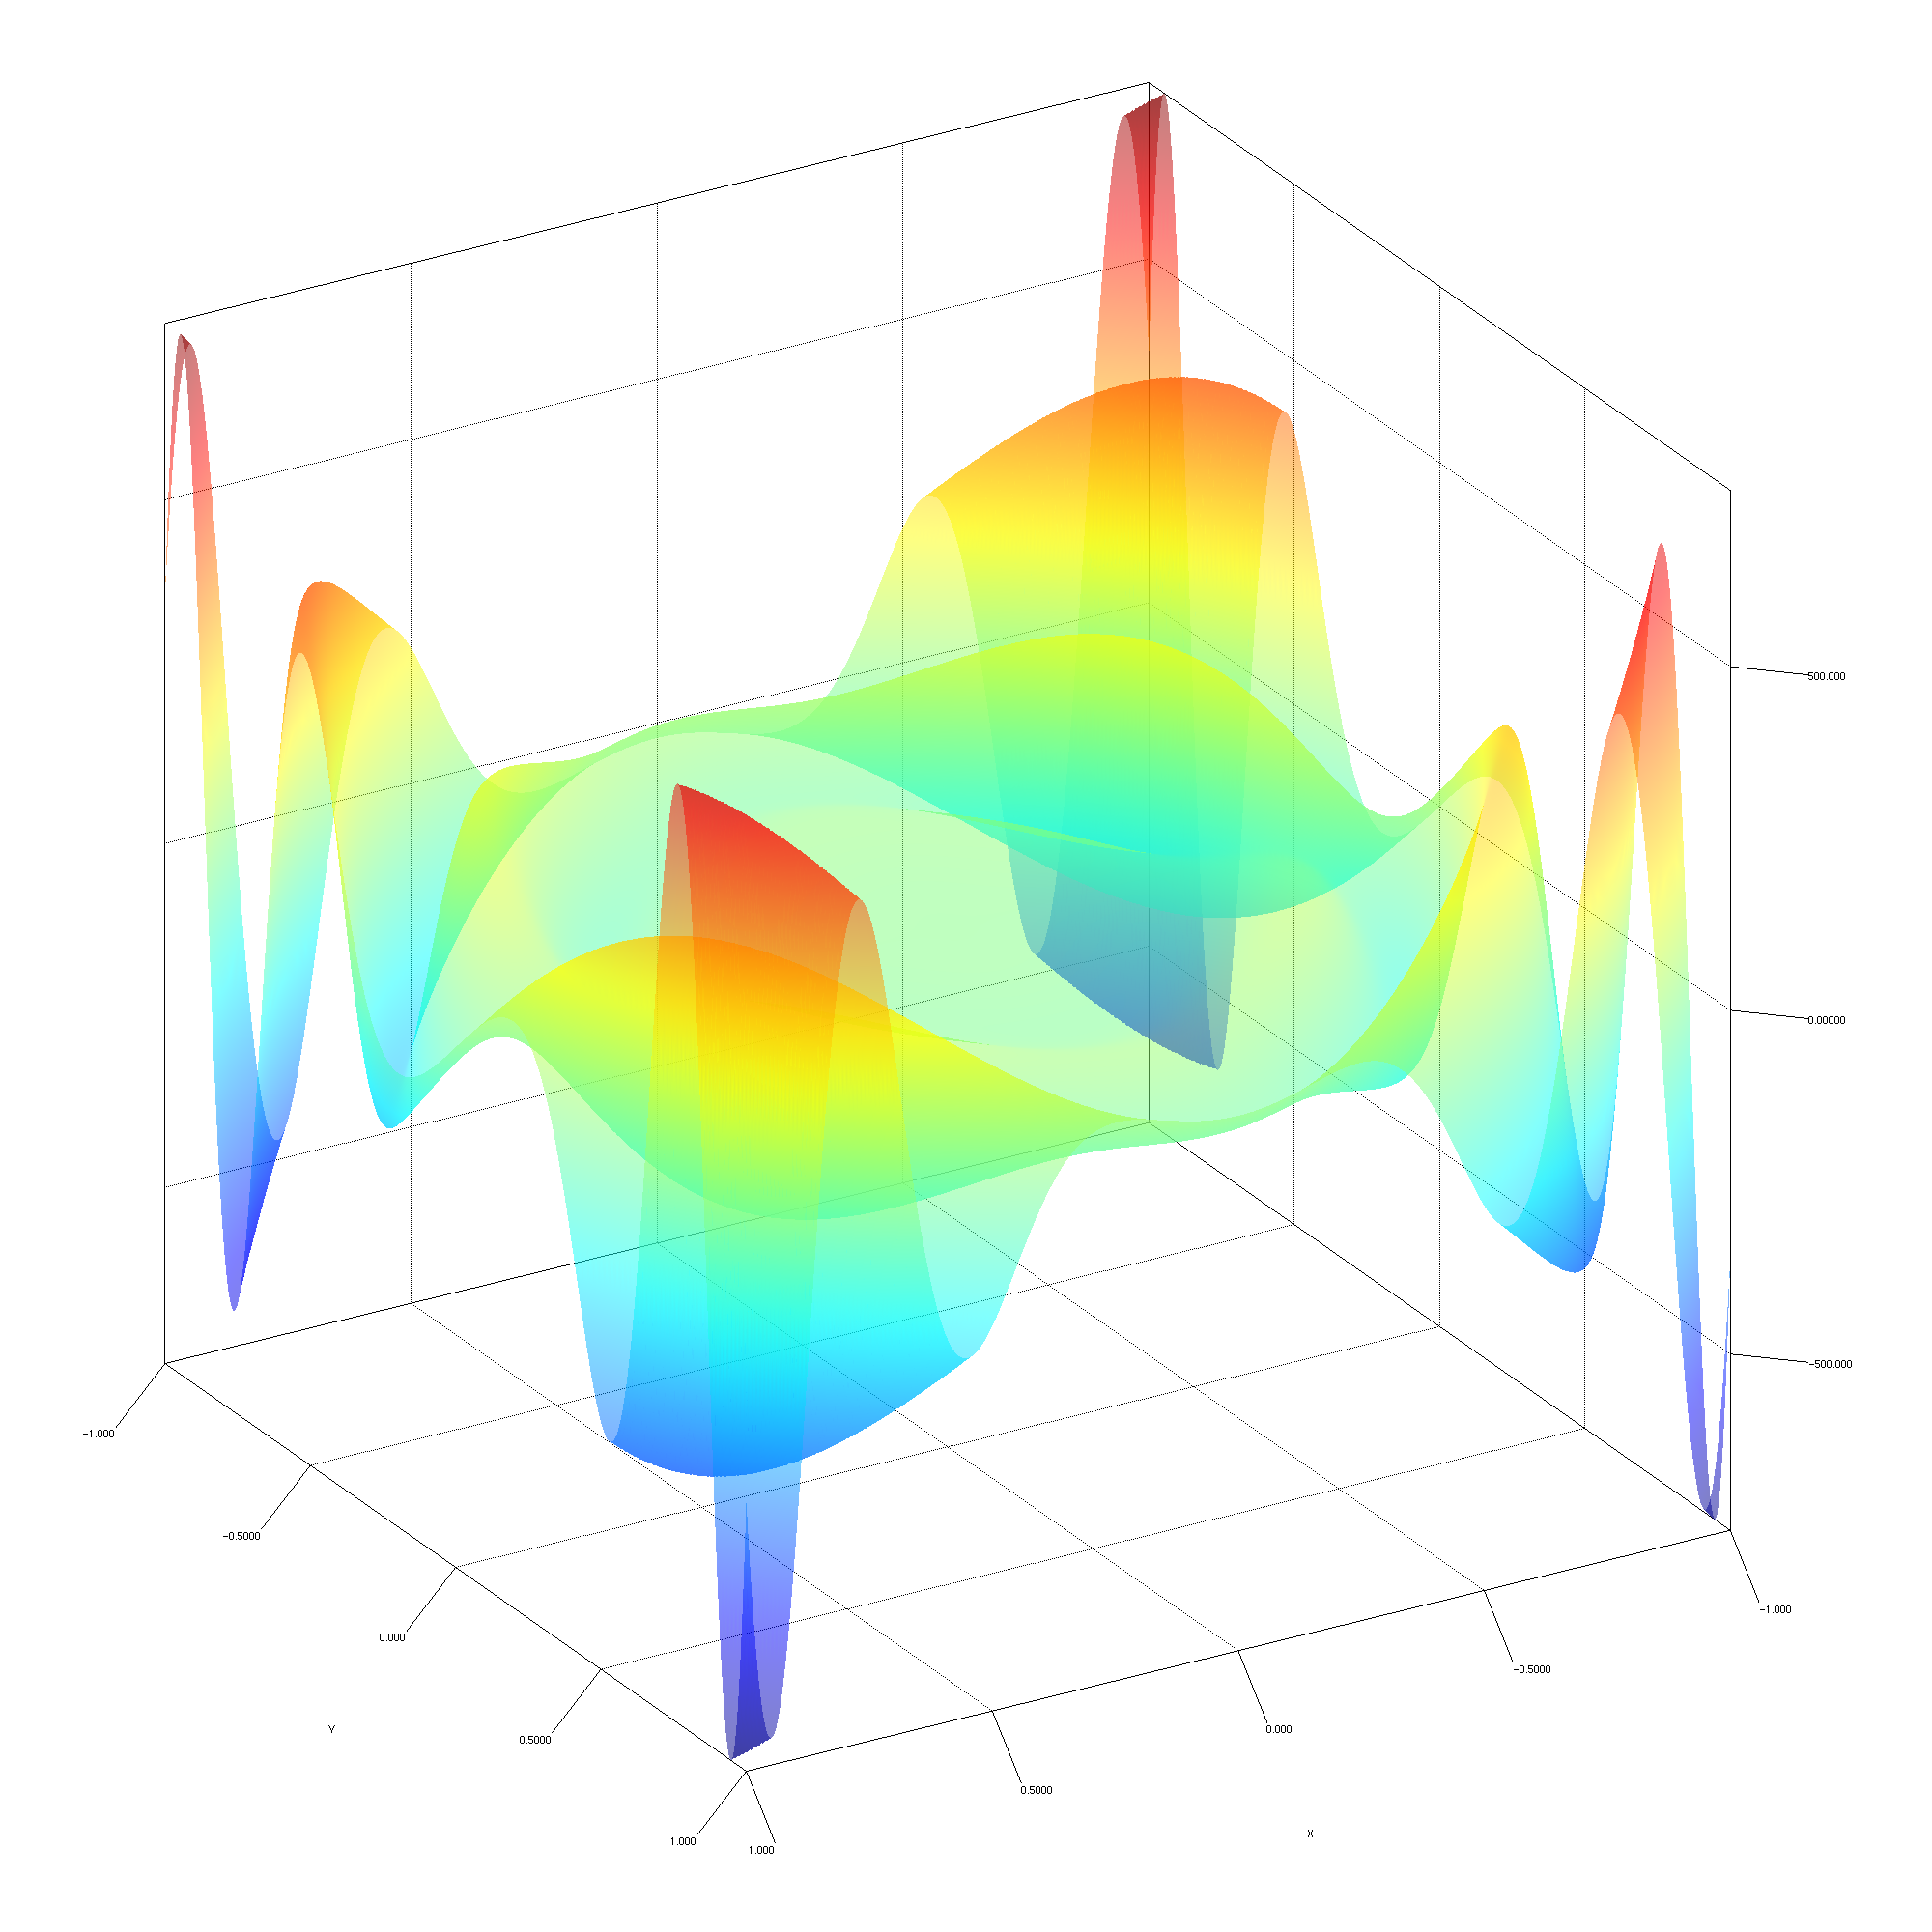
\includegraphics[scale=0.43]{plot_result.png}
\squeezeup\caption{Output generated by the program shown in Figure \ref{label:fig1}.}\squeezeup
\end{figure}

Kotlin$\nabla$ treats mathematical functions and programming functions with the same underlying abstraction. Expressions are composed recursively to form a data-flow graph (DFG). An expression is simply a \texttt{Function}, which is only evaluated once invoked with numerical values, e.g. \texttt{z(0, 0)}.

\squeezeup\begin{figure}[!htb]
\begin{minted}[fontsize=\footnotesize]{kotlin}
val z = sin(10 * (x * x + pow(y, 2))) / 10
\end{minted}
\squeezeup\centering
\begin{tikzpicture}[grow=left]
\tikzset{level distance=45pt,sibling distance=-3pt}\squeezeup\squeezeup
\Tree [.$\div$ [.\texttt{sin} [.$\times$ \texttt{10} [.$+$ [.$\times$ \texttt{\textbf{x}} \texttt{\textbf{x}} ] [.\texttt{pow} \texttt{\textbf{y}} \texttt{2} ] ] ] ] \texttt{10} ]
\end{tikzpicture}
\squeezeup\squeezeup\squeezeup\caption{Implicit DFG constructed by the original expression, \texttt{z}.}
\end{figure}

\squeezeup Kotlin$\nabla$ supports shape-shafe tensor operations by encoding tensor rank as a parameter of the operand's type signature. By enumerating type-level integer literals, we can define tensor operations just once using the highest literal, and rely on Liskov substitution to preserve shape safety for subtypes.

\begin{figure}[!htb]
\begin{minted}[fontsize=\scriptsize]{kotlin}
// Literals have reified values for runtime comparison
open class `0`(override val value: Int = 0): `1`(0)
open class `1`(override val value: Int = 1): `2`(1)
class `2`(open val value: Int = 2) // Greatest literal
// <L: `2`> will accept L <= 2 via Liskov substitution
class Vec<E, L: `2`>(len: L, cts: List<E> = listOf())
// Define addition for two vectors of type Vec<Int, L>
operator scalarFun <L: `2`, V: Vec<Int, L>> V.plus(v: V) =
  Vec<Int, L>(len, cts.zip(v.cts).map { it.l + it.r })
// Type-checked vector addition with shape inference
val Y = Vec(`2`, listOf(1, 2)) + Vec(`2`, listOf(3, 4))
val X = Vec(`1`, listOf(1, 2)) + Vec(`3`) // Undefined!
\end{minted}
\squeezeup\squeezeup\caption{Shape safe tensor addition for rank-1 tensors, $\forall L\leq2.$}\squeezeup
\end{figure}

It is possible to enforce shape-safe vector construction as well as checked vector arithmetic up to a fixed \texttt{L}, but the full implementation is omitted for brevity. A similar pattern can be applied to matrices and higher rank tensors, where the type signature encodes the shape of the operand at runtime.

With these basic ingredients, we have almost all the features necessary to build an expressive shape-safe AD, but unlike prior implementations using Scala or Haskell, in a language that is fully interoperable with Java, while also capable of compiling to JVM bytecode, JavaScript, and native code.

In future work, we intend to implement a full grammar of differentiable primitives including matrix convolution, control flow and recursion. While Kotlin$\nabla$ currently implements arithmetic manually, we plan to wrap a BLAS such as cuBLAS or native linear algebra library for performance.

\squeezeup\bibliography{example_paper}
\bibliographystyle{sysml2019}

\end{document}